% ─────────────────────────────────────────────────────────────────────────────
% HOJA DE RESPUESTAS — PRIMARIA · 60 preguntas A-D · VERSIÓN 2
%
% Todo se dibuja con coordenadas ABSOLUTAS en mm desde la esquina superior
% izquierda de la hoja carta (215.9 x 279.4 mm), con "y" hacia abajo. El
% perfil OMR 'PRIMARIA60V2' (exam_profiles.py) se CALCULA de estas medidas.
%
% Guías OMR:
%   · 4 marcadores ArUco (DICT_4X4_50, ids 0-3) de 12 mm en las esquinas.
%     Cada uno es distinto: el lector sabe cuál es cuál, endereza la foto
%     aunque venga al revés o de lado, y avisa si falta alguno.
%     El rectángulo que forman sus bordes exteriores, (8,8)-(207.9,266.7) mm,
%     se mapea al lienzo 1275x1650 del lector (misma proporción).
%   · 1 marca negra por fila a la izquierda de cada columna (ubican las filas)
%
% Compilar 2 veces:  pdflatex primaria_60_v2.tex
% ─────────────────────────────────────────────────────────────────────────────
\documentclass[letterpaper]{article}
\usepackage[margin=0pt]{geometry}
\usepackage[T1]{fontenc}
\usepackage[utf8]{inputenc}
\usepackage{helvet}
\usepackage{graphicx}
\usepackage{tikz}
\usetikzlibrary{calc}
\renewcommand{\familydefault}{\sfdefault}
\pagestyle{empty}
\setlength{\parindent}{0pt}

% ── Geometría (mm) — si cambia, recalcular el perfil PRIMARIA60V2 ────────────
\def\Brad{3.5}        % radio de la burbuja  → 7 mm de diámetro
\def\RowPitch{9.45}   % distancia entre filas
\def\OptPitch{10.5}   % distancia entre opciones A-B-C-D
\def\RowOne{64.5}     % y del centro de la fila 1
\def\BoxTop{52.5}     % borde superior de las cajas de respuestas
\def\BoxBot{250.5}    % borde inferior
\def\BoxW{61}         % ancho de cada caja
\def\LetY{57.8}       % y de las letras A B C D sobre cada columna

% Caja de 20 preguntas.  #1 = x del borde izquierdo,  #2 = primera pregunta
\newcommand{\Columna}[2]{%
  \draw[rounded corners=3mm, line width=0.9pt, black!75]
        (#1,\BoxTop) rectangle (#1+\BoxW,\BoxBot);
  % letras de encabezado
  \foreach \opt/\k in {A/0,B/1,C/2,D/3}{
    \node[font=\bfseries\fontsize{13}{13}\selectfont]
         at (#1+23+\k*\OptPitch,\LetY) {\opt};
  }
  \foreach \r in {0,...,19}{
    \pgfmathsetmacro{\yy}{\RowOne+\r*\RowPitch}
    \pgfmathtruncatemacro{\num}{#2+\r}
    % marca de fila (timing mark): 3.5 x 4.5 mm
    \fill[black] (#1+3,\yy-2.25) rectangle (#1+6.5,\yy+2.25);
    % número de pregunta
    \node[anchor=east, inner sep=0pt, font=\bfseries\fontsize{12}{12}\selectfont]
         at (#1+17,\yy) {\num.};
    % burbujas con su letra en gris claro
    \foreach \opt/\k in {A/0,B/1,C/2,D/3}{
      \draw[line width=0.75pt, black!75, fill=white]
           (#1+23+\k*\OptPitch,\yy) circle (\Brad);
      \node[inner sep=0pt, text=black!27,
            font=\bfseries\fontsize{10}{10}\selectfont]
           at (#1+23+\k*\OptPitch,\yy) {\opt};
    }
  }
  % separador cada 5 preguntas (ayuda a no perder la fila)
  \foreach \g in {5,10,15}{
    \pgfmathsetmacro{\ys}{\RowOne+(\g-0.5)*\RowPitch}
    \draw[line width=0.5pt, black!40] (#1+8.5,\ys) -- (#1+\BoxW-2.5,\ys);
  }
}

% Marcador ArUco de 6x6 módulos de 2 mm.  #1,#2 = esquina superior izquierda
% (mm),  #3 = los 36 bits por filas (1 = negro).  NO cambiar tamaño ni bits.
\newcommand{\Marcador}[3]{%
  \fill[black] (#1,#2) rectangle (#1+12,#2+12);
  \foreach \bit [count=\i from 0] in {#3}{
    \ifnum\bit=0
      \pgfmathtruncatemacro{\cc}{mod(\i,6)}
      \pgfmathtruncatemacro{\rr}{int(\i/6)}
      \fill[white] (#1+\cc*2,#2+\rr*2) rectangle (#1+\cc*2+2,#2+\rr*2+2);
    \fi
  }
}

\begin{document}
\begin{tikzpicture}[remember picture, overlay]
\begin{scope}[shift={(current page.north west)}, x=1mm, y=-1mm]

  % ── 4 MARCADORES DE ESQUINA (no mover: los usa el escáner) ───────────────
  %    id 0 = arriba-izq, 1 = arriba-der, 2 = abajo-der, 3 = abajo-izq
  \Marcador{8}{8}        {1,1,1,1,1,1,1,0,1,0,0,1,1,1,0,1,0,1,1,1,1,0,0,1,1,1,1,0,1,1,1,1,1,1,1,1}
  \Marcador{195.9}{8}    {1,1,1,1,1,1,1,1,1,1,1,1,1,0,0,0,0,1,1,0,1,1,0,1,1,0,1,0,1,1,1,1,1,1,1,1}
  \Marcador{195.9}{254.7}{1,1,1,1,1,1,1,1,1,0,0,1,1,1,1,0,0,1,1,1,1,0,1,1,1,0,0,1,0,1,1,1,1,1,1,1}
  \Marcador{8}{254.7}    {1,1,1,1,1,1,1,0,1,1,0,1,1,0,1,1,0,1,1,1,0,1,1,1,1,1,0,0,1,1,1,1,1,1,1,1}

  % ── ENCABEZADO ───────────────────────────────────────────────────────────
  \draw[rounded corners=3mm, line width=1.2pt] (24,8) rectangle (192,41);
  \node[inner sep=0pt] at (38,24.5)
       {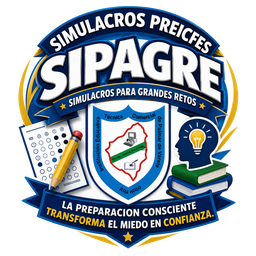
\includegraphics[width=25mm]{../static/sipagre_logo_sm.png}};
  \node[anchor=west, inner sep=0pt, font=\bfseries\fontsize{13}{14}\selectfont]
       at (54,14.2) {SIPAGRE · SIMULACRO PARA GRANDES RETOS};
  % insignia PRIMARIA
  \fill[black, rounded corners=2.2mm] (161.5,10.4) rectangle (189,18);
  \node[text=white, inner sep=0pt, font=\bfseries\fontsize{11}{12}\selectfont]
       at (175.25,14.2) {PRIMARIA};

  % líneas para escribir (altas, para letra de niño)
  \draw[line width=0.8pt] (54,27) -- (189,27);
  \node[anchor=north west, inner sep=0pt, font=\bfseries\fontsize{7.5}{8}\selectfont]
       at (54,28) {NOMBRES Y APELLIDOS};
  \draw[line width=0.8pt] (54,36.5) -- (118,36.5);
  \node[anchor=north west, inner sep=0pt, font=\bfseries\fontsize{7.5}{8}\selectfont]
       at (54,37.5) {DOCUMENTO DE IDENTIDAD};
  \draw[line width=0.8pt] (124,36.5) -- (152,36.5);
  \node[anchor=north west, inner sep=0pt, font=\bfseries\fontsize{7.5}{8}\selectfont]
       at (124,37.5) {CURSO};
  \draw[line width=0.8pt] (158,36.5) -- (189,36.5);
  \node[anchor=north west, inner sep=0pt, font=\bfseries\fontsize{7.5}{8}\selectfont]
       at (158,37.5) {FECHA};

  % ── INSTRUCCIÓN CON EJEMPLOS ─────────────────────────────────────────────
  \node[anchor=west, inner sep=0pt, font=\fontsize{10.5}{11}\selectfont]
       at (13,47) {\textbf{Rellena TODO el círculo} con lápiz. Si te equivocas, borra muy bien.};
  \node[anchor=east, inner sep=0pt, font=\bfseries\fontsize{10.5}{11}\selectfont]
       at (139,47) {Así sí:};
  \fill[black!88] (144,47) circle (2.6);
  \node[anchor=east, inner sep=0pt, font=\bfseries\fontsize{10.5}{11}\selectfont]
       at (166,47) {Así no:};
  % equis
  \draw[line width=0.6pt, black!75] (171,47) circle (2.6);
  \draw[line width=0.9pt] (169.3,45.3) -- (172.7,48.7) (169.3,48.7) -- (172.7,45.3);
  % chulo
  \draw[line width=0.6pt, black!75] (179,47) circle (2.6);
  \draw[line width=0.9pt] (177.3,47.2) -- (178.6,48.7) -- (181.2,45.2);
  % punto pequeño
  \draw[line width=0.6pt, black!75] (187,47) circle (2.6);
  \fill[black!88] (187,47) circle (0.9);
  % a medias
  \draw[line width=0.6pt, black!75] (195,47) circle (2.6);
  \begin{scope}
    \clip (195,47) circle (2.6);
    \fill[black!88] (192,47) rectangle (198,50);
  \end{scope}

  % ── RESPUESTAS: 3 columnas x 20 preguntas ────────────────────────────────
  \Columna{12}{1}
  \Columna{77.5}{21}
  \Columna{143}{41}

  % ── PIE ──────────────────────────────────────────────────────────────────
  \node[inner sep=0pt, font=\fontsize{8.5}{9}\selectfont, text=black!80]
       at (107.95,260.7)
       {No dobles ni arrugues la hoja \,·\, No rayes los cuadros de las esquinas ni las marcas de cada fila};

\end{scope}
\end{tikzpicture}
\end{document}
